%-------------------------------------------------------------------------------------------
			\subsubsection{Turning module}
%-------------------------------------------------------------------------------------------

\begin{figure}[t]
\centering
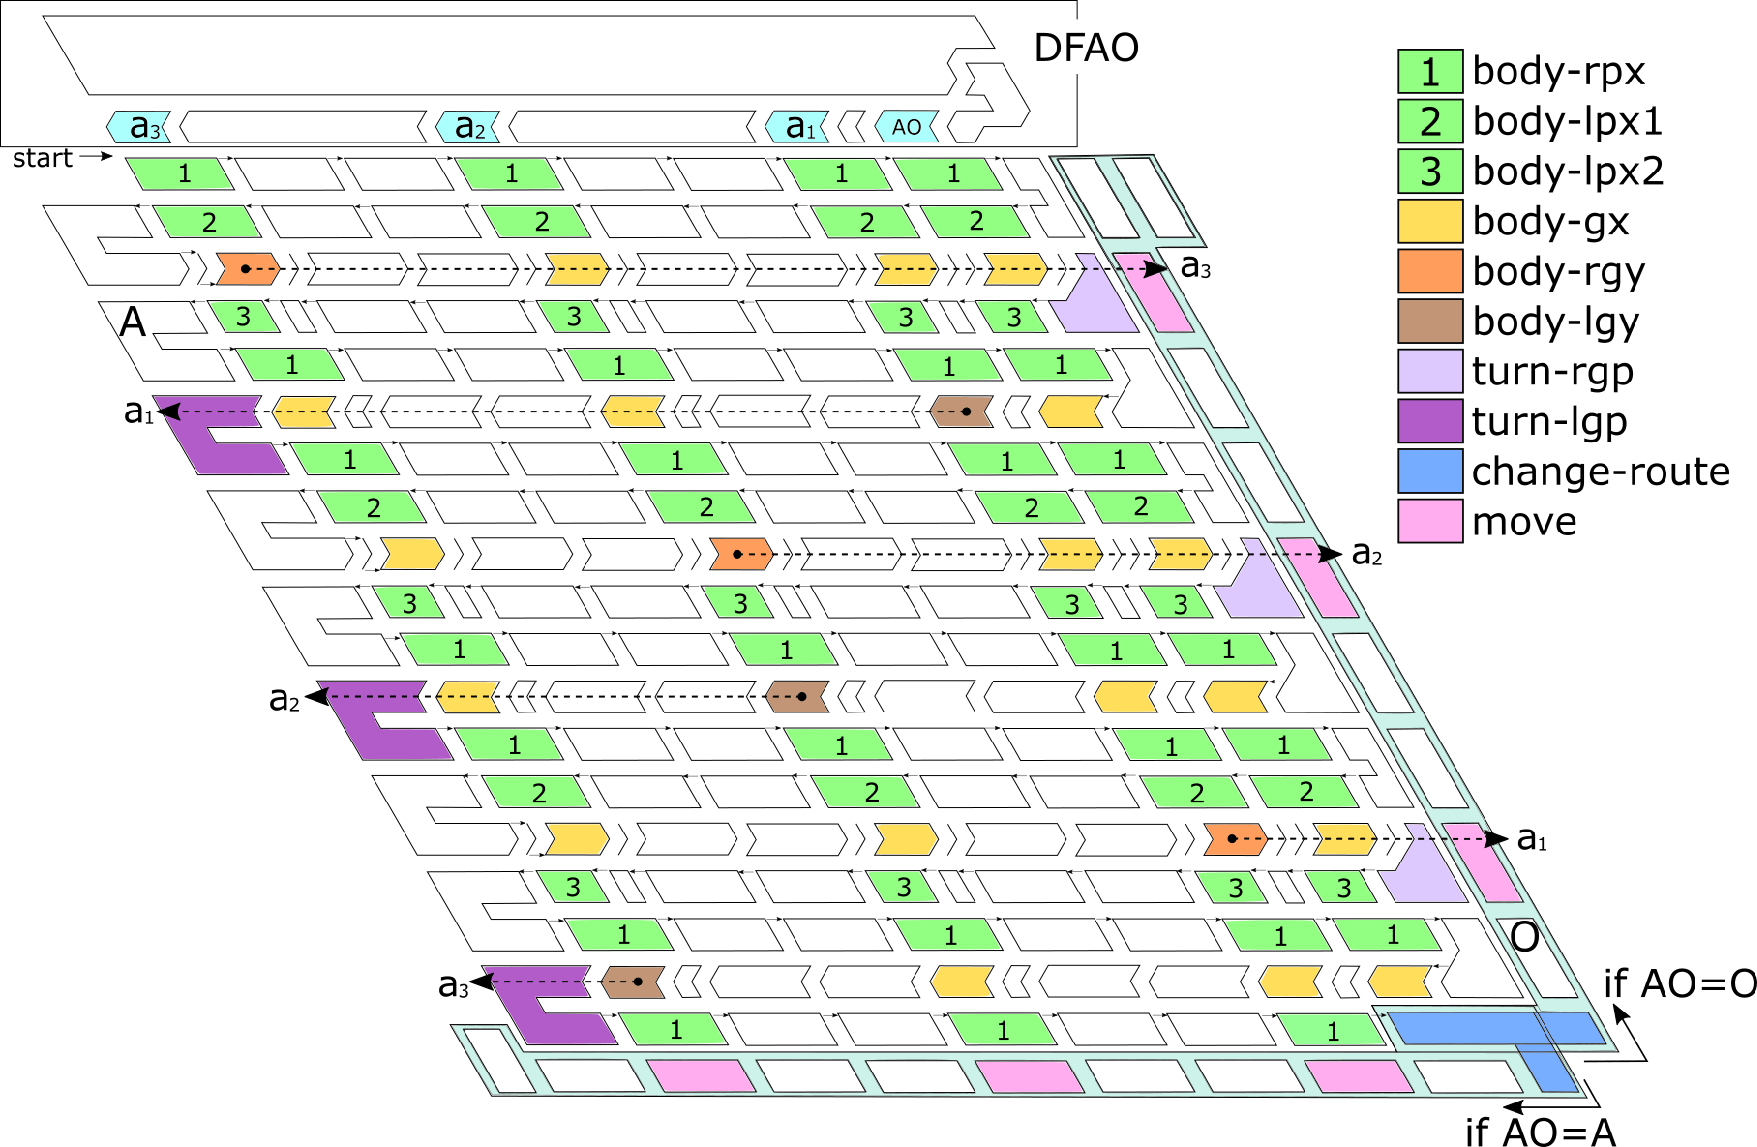
\includegraphics[width=\linewidth]{pic/overall_turn_part.pdf}
\caption{
Component-level abstraction of folding of turning module.
All the white components in the middle are spacers, some of which are implemented in the shape of parallelogram instead of glider. 
 }
\label{fig:overall_turning}
\end{figure}

The last module is for turn. 
It consists of two submodules: bit-sequence bifurcator and steering arm (shaded in light blue in Fig.~\ref{fig:overall_turning}). 

The bifurcator bifurcates the bits of the current count $i$ and the reinterpreted signal (A or O) as shown in Fig.~\ref{fig:abst_dragon} while folding into zigzags.
For that, it employs components to handle the following four types of tasks: 
\begin{enumerate}[itemsep=0pt]
\item propagate 1-bit vertically: body-rpx (Fig.~\ref{fig:body-rpx} (left)), body-lpx1 (Fig.~\ref{fig:body-rpx} (right)), and body-lpx2 (Fig.~\ref{fig:half-adder});
\item let 1-bit cross another 1-bit: body-gx (Fig.~\ref{fig:DFAO-zag2}); 
\item fork 1-bit vertically and horizontally: body-rgy (Fig.~\ref{fig:DFAO-zag2}) and body-lgy (Fig.~\ref{fig:body-lgy});  
\item undergo transition between a zig and a zag and exposes 1-bit outside: turn-rgp (Fig.~\ref{fig:turn-rgp}) and turn-lgp (Fig.~\ref{fig:turn-lgp}). 
\end{enumerate} 
%that propagates 1bit vertically (body-rpx, body-lpx1, and body-lpx2 in Figure~\ref{fig:overall_turning}), that lets 1bit cross another 1bit (body-gx), that forks 1bit vertically and horizontally (body-rgy, body-lgy), and that undergoes transition from a zig to a zag or from a zag to a zig and exposes 1bit outside (turn-rgp, turn-lgp).
Components to handle the first two types of tasks have already been implemented (see, e.g., \cite{HaKiOtSe2016}) so that we shall explain the others.

%The component body-rgy takes one of the two conformations in Figure~\ref{fig:body-rgy} depending on the 1-bit encoded in the two beads above.
%Output below, the 1-bit is encoded as a type of the second bead from left, while output right, it is encoded as the position of its last bead (top or bottom).
%Its zag-variant, body-lgy, is implemented analogously; for its conformations.

%\begin{figure}[h]
\begin{wrapfigure}{r}{0.55\linewidth}
\vspace*{-5mm}
\centering
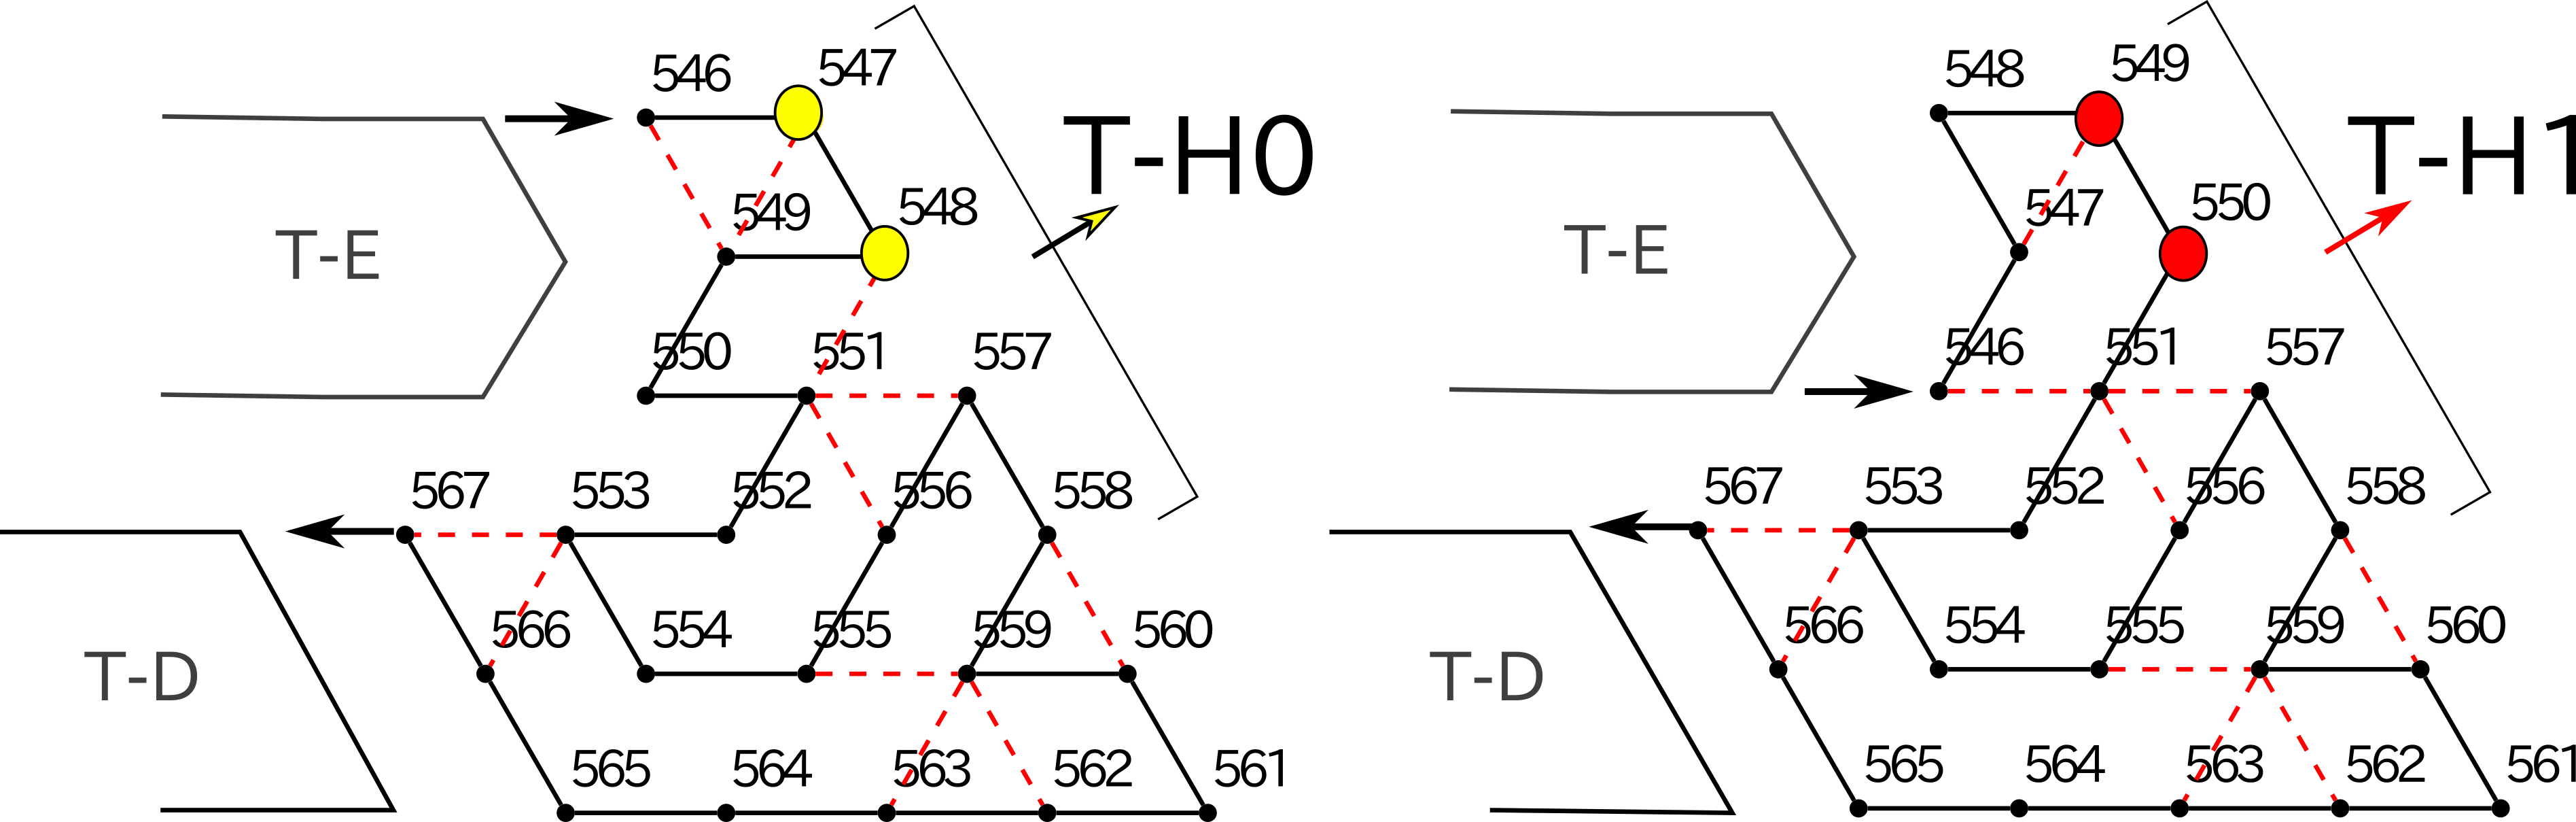
\includegraphics[width=\linewidth]{pic/turn-rgp.png}
\caption{The two conformations of turn-rgp.}
\label{fig:turn-rgp}
\vspace*{-3mm}
\end{wrapfigure}
%\end{figure}

The component body-rgy is implemented by reusing the first half of DFAO-zag2 (Fig.~\ref{fig:DFAO-zag2}). 
Starting from the bottom, it can take two conformations which end at different heights and expose sequences of bead types sufficiently pairwise distinct downward. 
Hence, we can divert it to fork 1bit input rightward and downward. 
The 1bit thus forked transfers till the end of a zag and is converted by the turn-rgp into a sequence of bead types (see Fig.~\ref{fig:turn-rgp}). 
The body-lgy and turn-lgp are their zig counterparts (Figs.~\ref{fig:body-lgy} and \ref{fig:turn-lgp}). 

%The 1bit forked rightward by a body-rgy transfers till the end of the zig without being jammed because all remaining modules in the zig are designed in such a way that they start and end at the same height like the even-distance glider.
%The module turn-rgp receives the 1bit (top or bottom), and exposes it by taking one of the two comformations in Figure~\ref{fig:turn-rgp}.
%The module turn-lgp functions analogously in zags as being folded in Figure~\ref{fig:turn-lgp}.

\begin{figure}[h]
\centering
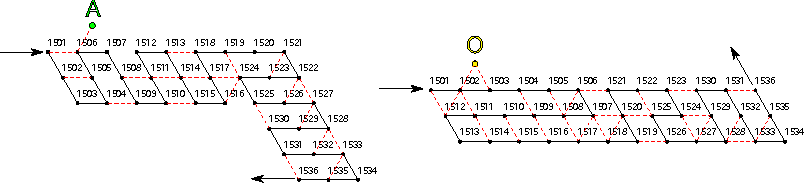
\includegraphics[width=\linewidth]{pic/change_route.pdf}
\caption{The two conformations of change-route.}
\label{fig:change_route}
\end{figure}

The bifurcator also propagates the 1-bit A/O, output by the DFAO module, to tell the steering arm which way it should take.
Specifically, the signal has the component, change-route, of the steering arm take one of the two conformations in Fig.~\ref{fig:change_route}, guiding the rest of the arm towards the specified direction.
The remaining arm is a catenation of move components (Fig.~\ref{fig:move}), which is capable of letting the bifurcated bit sequence through.  
Note that the turning module need not bifurcate AO.
Indeed, the second and third turning modules are supposed to turn in the same manner as the first one.
It hence suffices to append A and O to the bifurcated bit sequences on the acute side and obtuse side, respectively, as shown in Fig.~\ref{fig:overall_turning}.

\begin{remark}
As suggested in Fig.~\ref{fig:overall_turning}, the bifurcation component actually outputs an input bit sequence also downward.
That is, it trifurcates the input.
This provides a more space-efficient way to replicate a bit sequence many-folds.
\end{remark}

